\section{Video Synthesis}
\label{sec:video_synthesis}

\begin{figure}
    \centering
    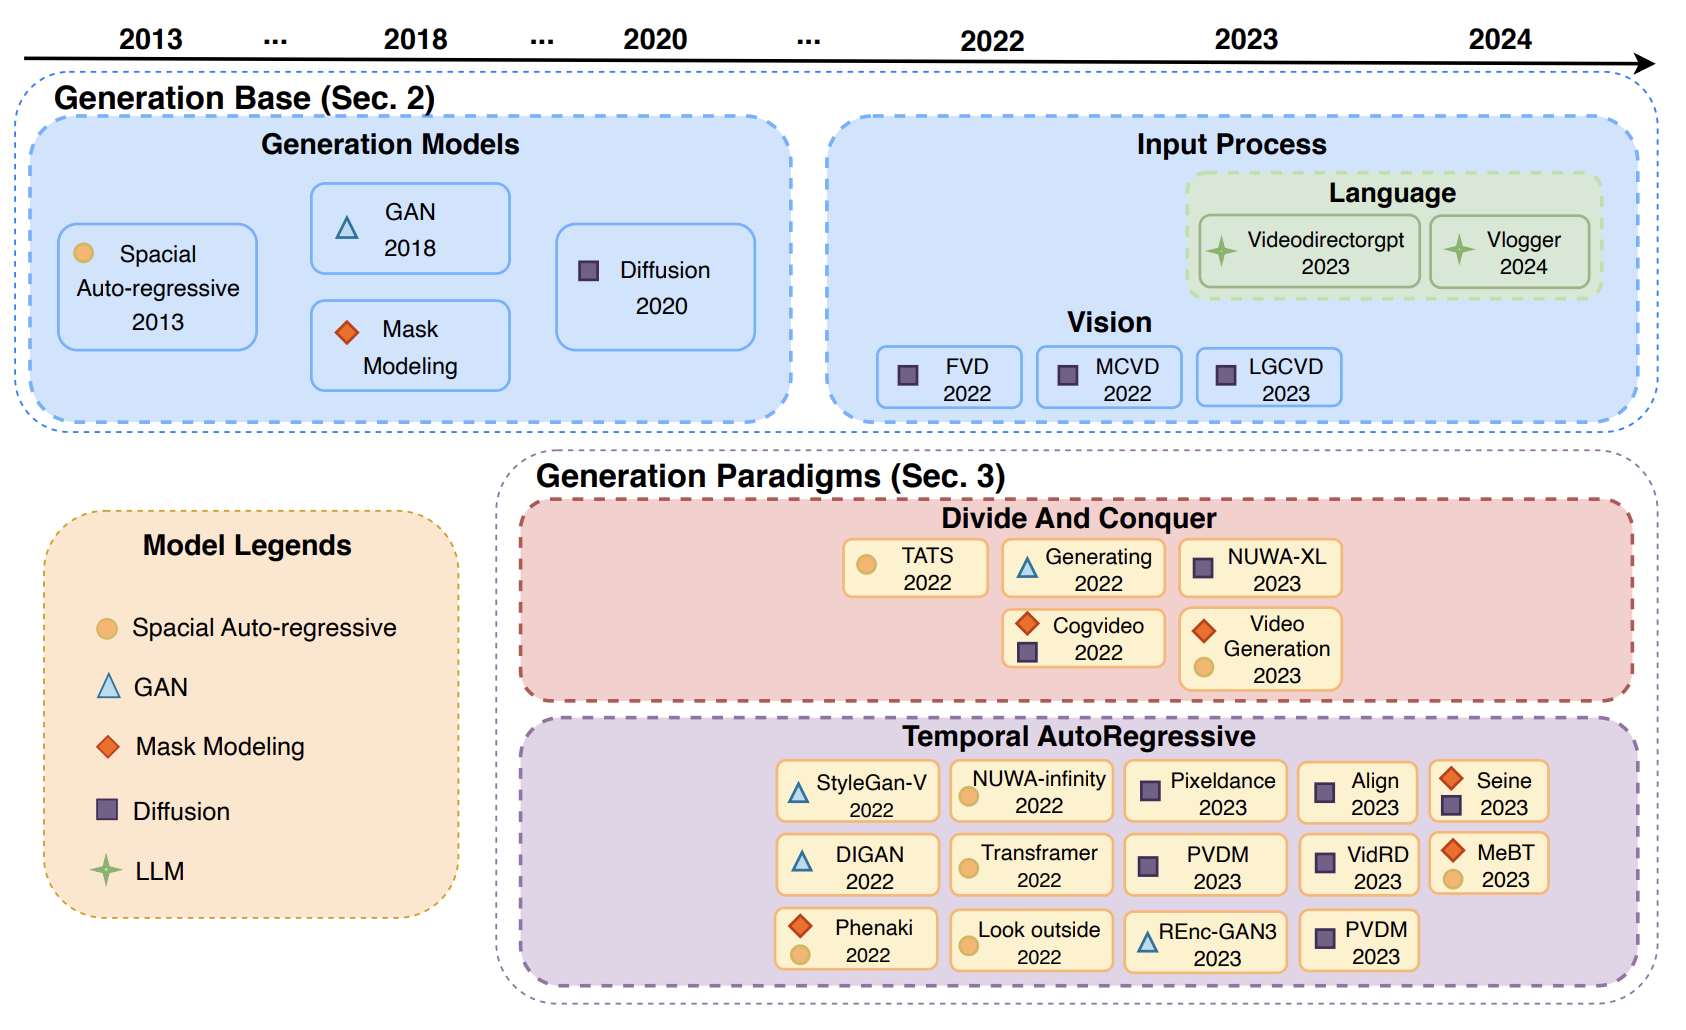
\includegraphics[width=0.7\textwidth]{images/video_synthesis/techniques.png}
    \caption{Overview of video synthesis techniques \cite{long_video_survey}.}
    \label{fig:video_synthesis_techniques}
\end{figure}

Video synthesis is a complex task. One can think of video generation as a sequence of image generation tasks. Formally, a video is a sequence of images (or frames) that are shown in fast fashion, usually 24 frames per second (at the minimum, to get smooth video). Therefor to create a video of 5 seconds, you'll need 120 frames or images at the minimum. Additional complexity is the addition of the \textbf{time dimension}, which is not present in image generation tasks. The video should be \textbf{coherent} in time, meaning that the frames should be related to each other and should follow a logical sequence. Objects should not appear out of nowhere, there should be \textbf{smooth transition of motion} and correct \textbf{spatial relationships} between objects. We also have to deal with limited hardware resources, since video generation is extremely computationally expensive.

% TODO: Add timeline of video synthesis models
% \begin{figure}
    \centering
    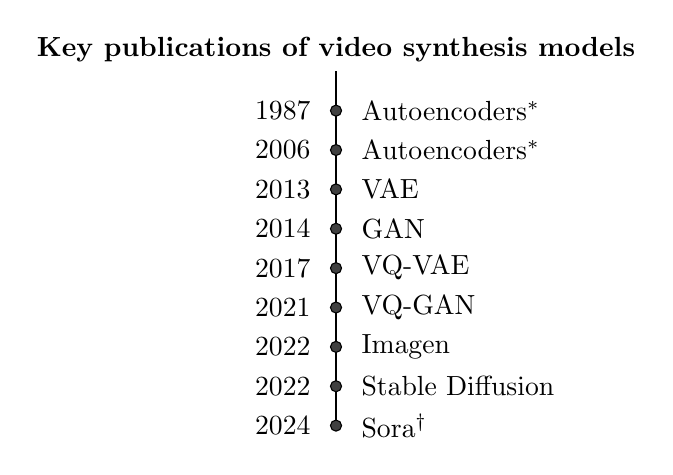
\begin{tikzpicture}
        \def\step{0.5} % step size for vertical spacing
        \def\numtimeline{9} % Number of events in the timeline

        % Define timeline line
        \draw[thick, color=black] (0,0) -- (0,-\numtimeline*\step);

        % Define timeline events with adjusted positions
        \foreach \i/\year/\text in 
        {
            1/1987/Autoencoders$^*$, 
            2/2006/Autoencoders$^*$, 
            3/2013/VAE, 
            4/2014/GAN, 
            5/2017/VQ-VAE,
            6/2021/VQ-GAN,
            7/2022/Imagen,
            8/2022/Stable Diffusion,
            9/2024/Sora$^\dag$
        } {
        \draw[fill=darkgray] (0,-\i*\step) circle (2pt);
        \node[anchor=east] at (-0.2,-\i*\step) {\year};
        \node[anchor=west] at (0.2,-\i*\step) {\text};
        }

        % Define timeline title
        \node[anchor=south] at (0,0) {\textbf{Key publications of video synthesis models}};
    \end{tikzpicture}
    \caption{Chronology of key video generation models publications.}
  \end{figure}

% There are a lot of techniques and models for video generation, and they can be divided into multiple categories:

% \begin{itemize}
%     \item \textbf{Frame prediction}: ...
%     \item \textbf{GAN based models}: such in the case of \cite{chu2020learning} the authors propose 
% \end{itemize}

Video synthesis can be based on four main models and methods:

\begin{enumerate}
    \item \textbf{Diffusion}: diffusion models for video generation extend the iterative refinement process used in image-based diffusion models, such as LDMs, to handle temporal dynamics required for videos. The key idea is to generate not just a sequence of independent images, but a continuous video where both the spatial content of each frame and the temporal coherence between frames are learned and generated simultaneously.
    \item \textbf{Spatial autoregressive}: spatial autoregressive models for video generation, as described in \cite{graves2013generating}, synthesize video by sequentially generating content in a patch-based fashion, where each patch in a frame is conditioned on previously generated patches. This method builds video frame-by-frame, ensuring spatial and temporal coherence across the entire sequence.
    \item \textbf{GAN}: similar to diffusion models, GANs can also be leveraged for video synthesis. 
    \item \textbf{Mask modeling}: mask modeling in video generation uses the technique of selectively masking parts of video frames during training to enhance the model's ability to learn spatial and temporal dependencies. By hiding portions of the video frames, the model is tasked with predicting and reconstructing the missing parts, forcing it to better understand the underlying structure and motion in the video.
\end{enumerate}

\begin{figure}
    \centering
    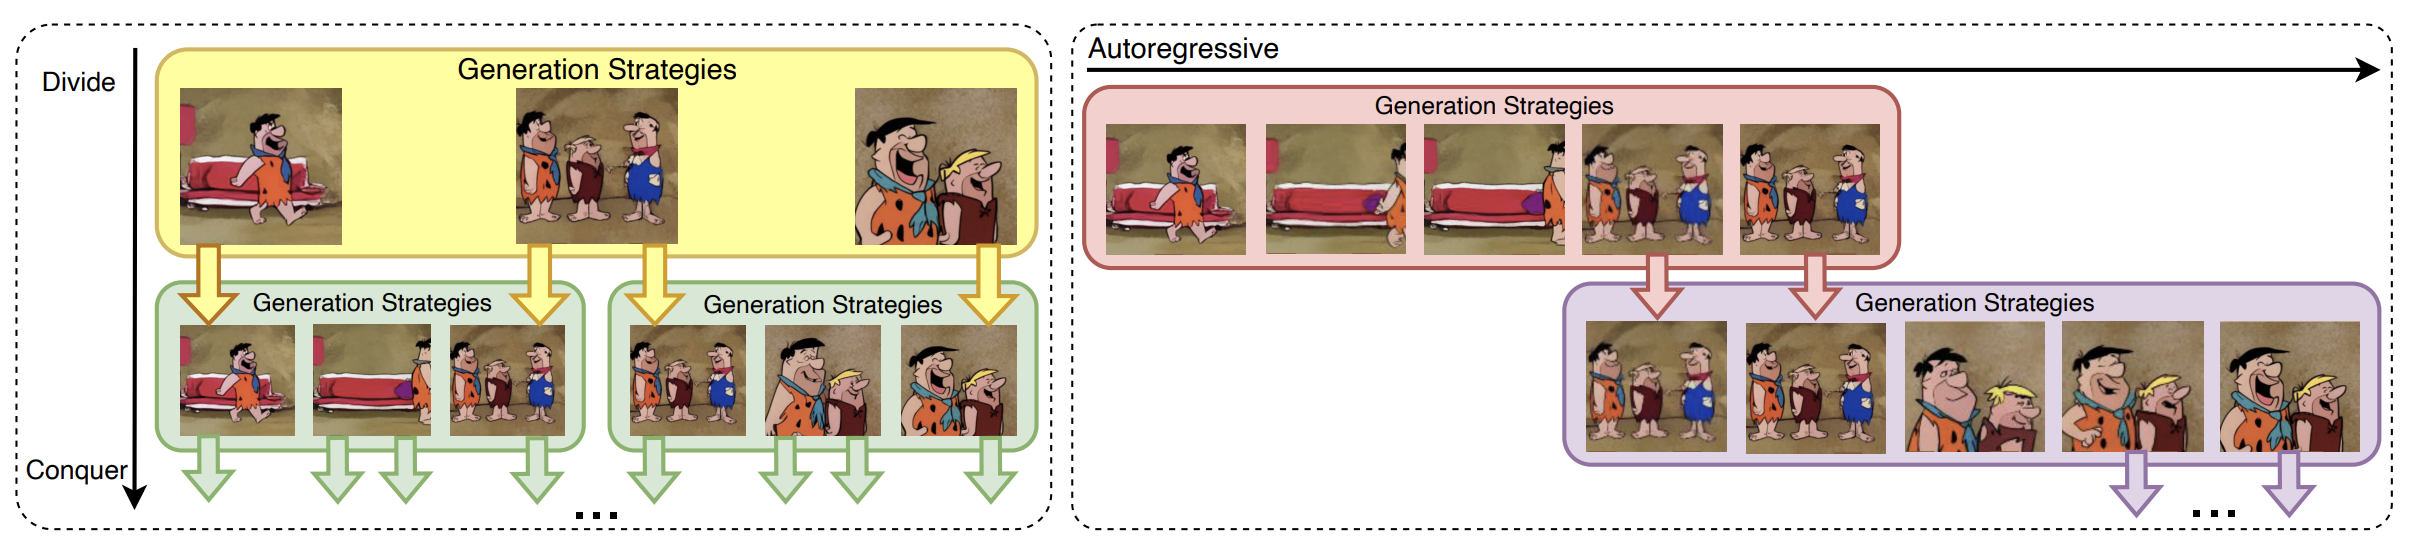
\includegraphics[width=1\textwidth]{images/video_synthesis/paradigms.png}
    \caption{Overview of video synthesis paradigms \cite{long_video_survey}. Divide and conquer is split into hierarchical architecture for keyframe generation and frame filling. Whereas temporal autoregressive paradigm the next frame prediction depends on the previous frame/frames.}
    \label{fig:video_synthesis_paradigms}
\end{figure}

In the realm of video synthesis there are two paradigms: \textbf{divide and conquer} and \textbf{temporal autoregressive}. An overview of the paradigms is shown in figure \ref{fig:video_synthesis_paradigms}.


\begin{figure}
    \centering
    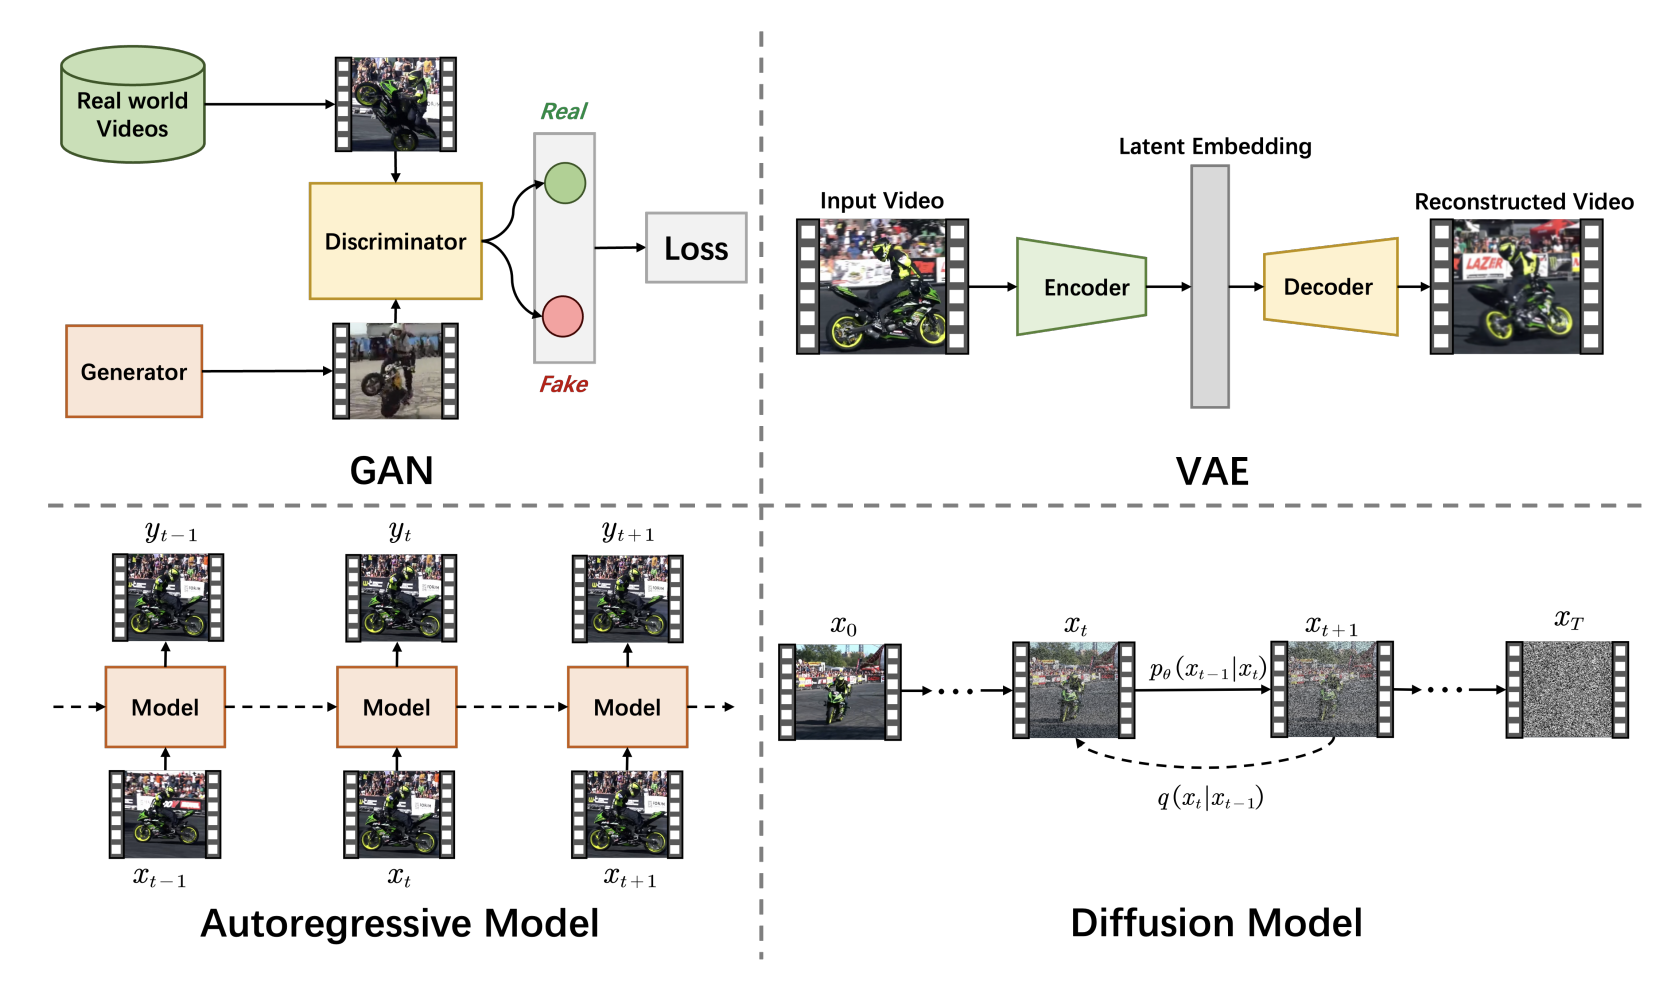
\includegraphics[width=0.6\textwidth]{images/video_synthesis/generation_technologies.png}
    \caption{An overview of video generation technologies: \textit{GAN:} based on adversarial loss and uses generator and discriminator; \textit{VAE:} compresses the input data in the encoder to lower dimension latent space and then learns to reconstruct the data in the decoder; \textit{Autoregressive:} frame by frame prediction; \textit{Diffusion:} the model adds noise and learns to remove noise with U-Net.}
\end{figure}


\subsection*{Divide and Conquer}

Divide and conquer paradigm breaks the task of video synthesis into smaller, more manageable tasks. This approach can further by divided into 3 methods of approach:

\begin{enumerate}
    \item \textbf{Hierarchical architecture for frame generation}: in this approach, the process is split into \textbf{keyframe generation} and \textbf{frame filling}. Keyframes represent the critical moments of the video that establish the narrative, while the frame-filling models ensure smooth transitions between them. Global models focus on generating the main storyline through keyframes, and local models handle finer details, filling the gaps between the keyframes to maintain temporal consistency.
    \item \textbf{Multi-stage approach for video super-resolution}: \cite{brooks2022generating} suggested generating video by stages, first by creating low-resolution sequences with GAN and then applying super-resolution models to enhance them with StyleGAN3 \cite{stylegan3}.
    % TODO: Explain the combined process of mask modeling, I don't really understand. Maybe read the paper CogVideo?
    \item \textbf{Integrated keyframe and frame filling with mask modeling} simplifies long video generation by combining keyframe creation and frame filling into a unified process. Mask modeling hides specific parts of the video during training, keyframes and intermediate frames simultaneously, like done in CogVideo \cite{cogvideo}, which simplified mask modeling and combines these models into a single model.
\end{enumerate}

\subsection*{Temporal autoregressive}

Temporal autoregressive paradigm is an iterative approach where each frame is generated based on the previous one. The model is trained on sequences of video data, and the output from one timestep serves as the input for the next (the next frame is conditioned on the previous frame, which in theory ensures that the video is temporally coherent).

A significant amount of research has been conducted on temporal autoregressive models, leading to various improvement strategies and enhancements for this framework. Some of the most notable include:

\begin{itemize}
    \item \textbf{Latent space compression}: this method focuses on compressing videos to latent space to optimize computational needs. For example in \cite{zeng2024make} and \cite{gu2023reuse} they explored condensing video data into 3D latent. Compression aims to preserve essential features across dimensions to improve computational efficiency.
    \item \textbf{Incorporating temporal layers} to refine individual video clips. Advancements were made, such as integrating \textbf{temporal layers} (such as attention and convolutional layers) into diffusion models, like in VideoLDM \cite{video_ldm} and \cite{gu2023reuse}. These temporal layers help the model better understand the temporal dynamics of video data.
    \item \textbf{Dual-phase training \& reuse strategies}: dual-training is a training strategy where the model is first trained unconditionally, and then learn to conditionally generate video like in Projected Latent Video Diffusion Model (PVDM) \cite{pvdm}. Given the abundance of unlabeled video data on the web, it's easy to see why this process is attractive. Another method to boost the model's ability to replicate long video sequences is a \textbf{reuse strategy}, which iteratively adds and removes noise during training to simulate natural variability, like in \cite{gu2023reuse}.
\end{itemize}

\subsection*{Spatial autoregressive models}

Spatial autoregressive models are adept at processing tokenized sequence inputs (they include the transformer architecture) which enable the segmentation of video frames into patches. By integrating video data features with the autoregressive power of transformers, these models become more capable of capturing temporal dynamics. In this method, there are two main approaches:

\begin{itemize}
    \item \textbf{Frame tokenization}: like in NUWA-Infinity \cite{nuwa_infinity}, the researchers transform video frames into patches and combine them with spatial positional encodings for more efficient data handling. These autoregressive models, similar to LDMs, compress video data into latent space. Compression techniques like \textbf{Discrete Cosine Transform (DCT)} are used in Transframer \cite{transframer} and by using VQGAN, they convert the frames into latent tokens.
    \item \textbf{Scaling with attention mechanism}: architectural modifications were made by incorporating specialized blocks, such as attention mechanism blocks tailored for spatiotemporal data. For example, Transframer \cite{transframer} integrated temporal and spatial annotations (time-steps, camera viewport, etc.) through cross-attention.
\end{itemize}

\subsection*{Challenges in video synthesis}

Because video synthesis is still developing to this day and is a complex task, there are a lot of open questions to be asked:

\begin{itemize}
    \item How to generate long videos while maintaining high temporal cohesion?
    \item Would it be possible to generate videos in high resolution, with limited computational resources?
    \item How to train video generation models with abundant, unlabeled video data, such as YouTube? Are there any open datasets for video generation?
    \item How to generate videos from text, or other modalities? Is it possible to edit generated videos so it fits our artistic needs?
    \item What is considered a long video? Frame count (e.g., 512, 1024 frames)? Duration (e.g., 3, 5 minutes)?
    \item How we would trade off between resolution (high resolution) of generated video, duration (long), and spatial coherence (smooth motion and logical spatial relationships)? Can we achieve all three?
    \item How to deal with abrupt scene transitions? How to ensure smooth transitions between scenes?
    \item How to measure and evaluate temporal-spatial consistency between video generation models? How to tell if one clip is smoother and more coherent than the other?
\end{itemize}

In \cite{long_video_survey} they surveyed papers in the field of video generation and propose a definition for 'long' videos to exceed 10 seconds long, assuming frame rate of 10fps, or equivalently 100 frames.

\subsection{Evaluation metrics}

\begin{figure}
    \centering
    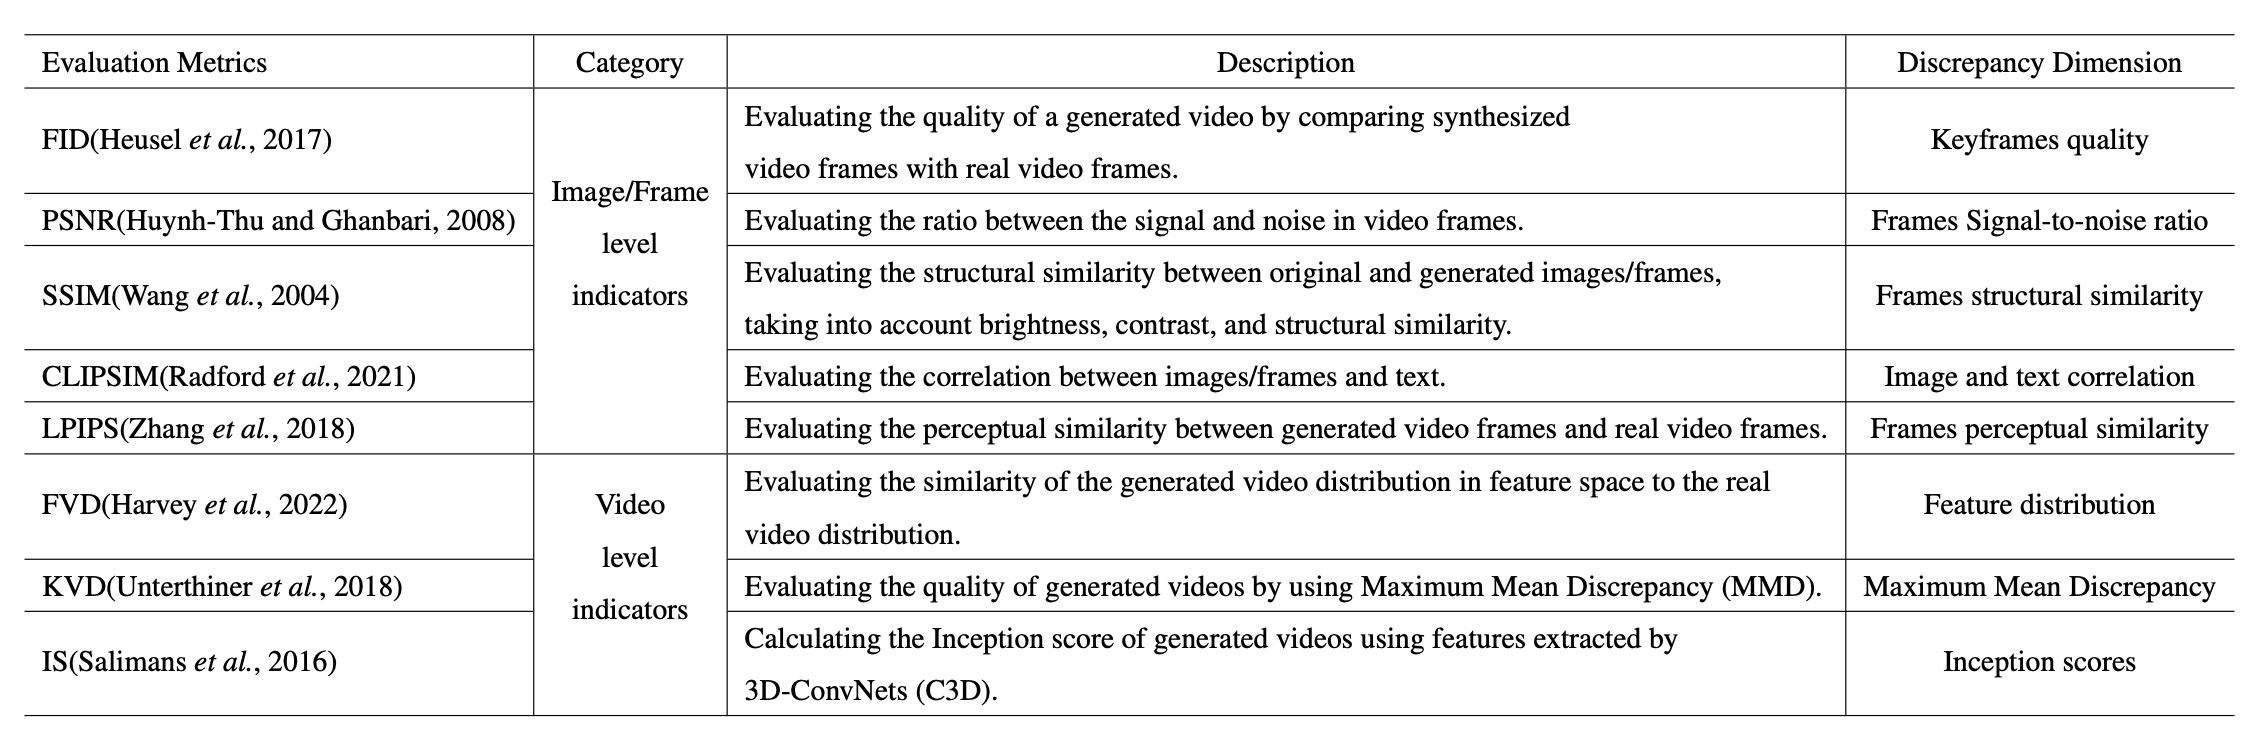
\includegraphics[width=1\textwidth]{images/video_synthesis/eval_metrics.png}
    \caption{Evaluation metrics in video generation \cite{long_video_survey}.}
    \label{fig:video_synthesis_eval_metrics}
\end{figure}

A common metric used for video generation models is the \textbf{Frechet Video Distance (FVD)} \cite{fvd}, which is an extension of Frechet Inception Distance (FID). FVD compares videos by both spatial and temporal features by using similar process as FID: using a pre-trained 3D ConvNet (i3D), where in FID they use InceptionV3. The i3D network was trained on Kinetics dataset (Kinetics Human Action Video Dataset), and the 3D convolutions capture local and global spatial patterns within the frames. In similar fashion as FID, they compare the distribution of features from generated videos and the FVD is calculated:

\begin{equation*}
    \text{FVD} = \left| \left| \mu_{\text{real}} - \mu_{\text{fake}} \right| \right|^2_2 + \text{Tr} \left( \Sigma_{\text{real}} + \Sigma_{\text{fake}} - 2 \left( \Sigma_{\text{real}} \Sigma_{\text{fake}} \right)^{1/2} \right)
\end{equation*}

The lower the FVD score, the better the video generation model is. A more comprehensive list of evaluation metrics is shown in figure \ref{fig:video_synthesis_eval_metrics}.

Although its not theoretically an evaluation metric, in the Diffusion Transformer (DiT) paper \cite{diffusion_transformer} the researchers used \textbf{Gflops} (giga floating point operations per second) metric to measure the complexity of the model, instead of traditional parameter count of the model. Higher Gflops means the model is more scalable and complex.



\subsection{Previous works}

\begin{figure}
    \centering
    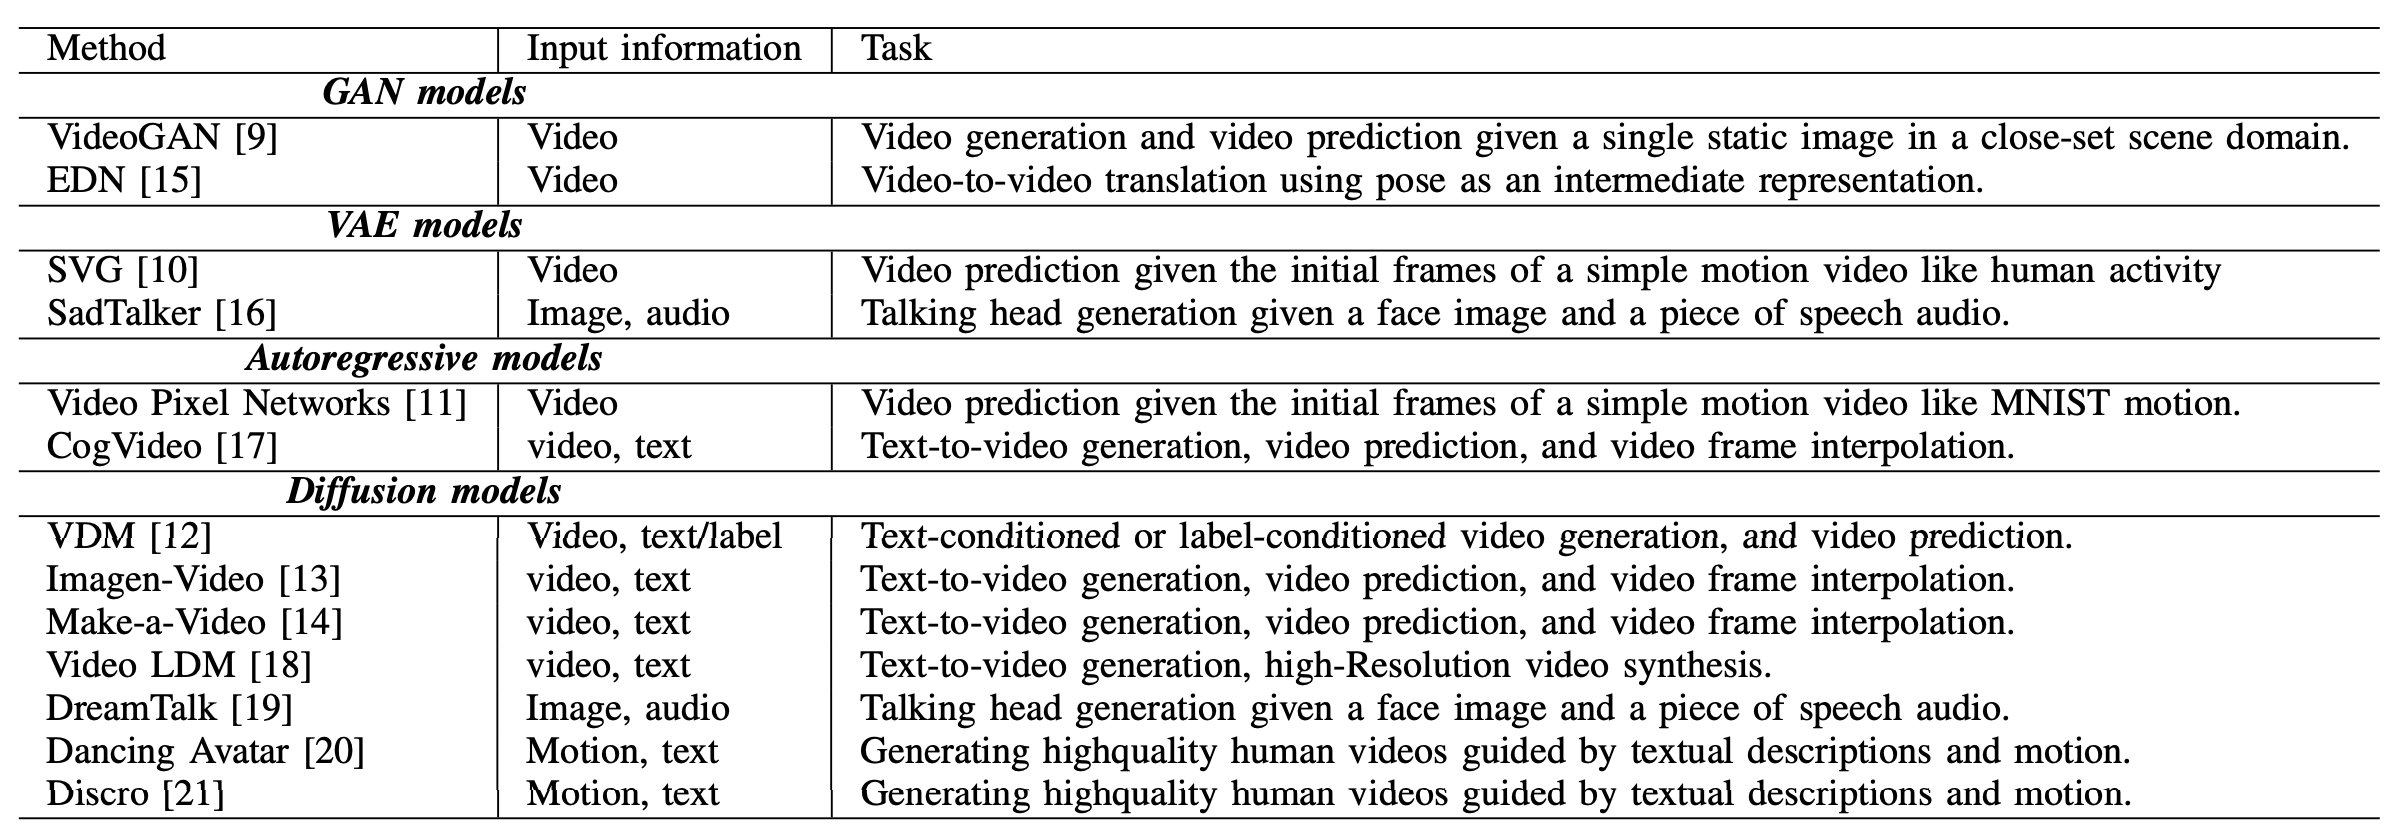
\includegraphics[width=0.7\textwidth]{images/video_synthesis/previous_works.png}
    \caption{Video generation models \& papers \cite{zhou2024survey}.}
\end{figure}

\begin{figure}
    \centering
    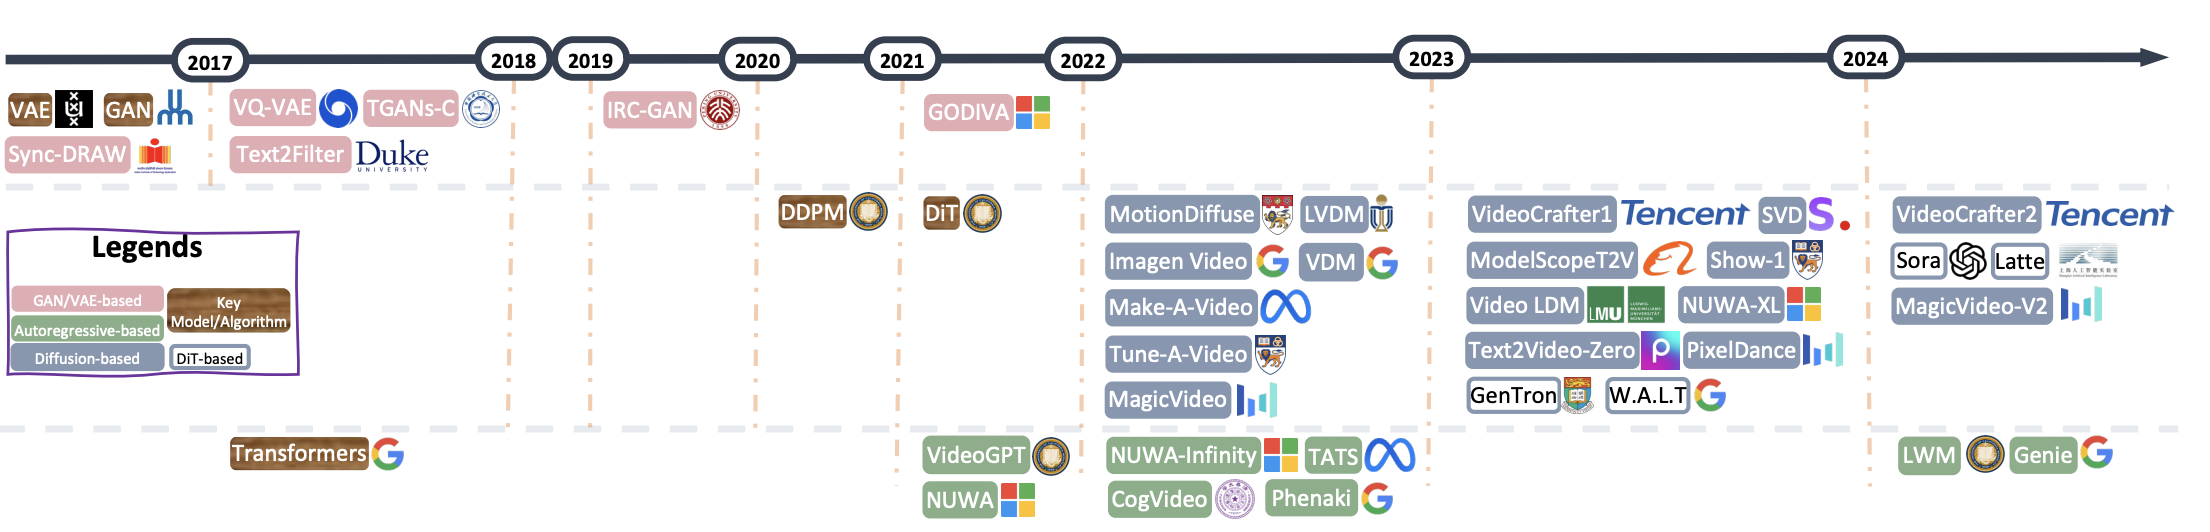
\includegraphics[width=1\textwidth]{images/video_synthesis/timeline.png}
    \caption{Text-to-Video generators evolutionary timeline, based on foundational algorithms \cite{sun2024sora}.}
\end{figure}

In \textbf{VideoGAN} \cite{video_gan} (2016) the researchers proposed to use of the large amounts of unlabeled video in order to learn scene dynamics and motion, and capture temporal signals. They proposed a model with \textbf{spatio-temporal convolutional} architecture, and they extend GANs to video generation. They successfully created a video of 1 second long, the model explicitly models the foreground separately from the background, which allows the network to learn which objects are in motion, and which don't. The methodology in this work is autoregressive frame prediction.

In the case of \cite{video_generation_from_text}, where the goal is to generate video from text, they proposed a hybrid model that uses a conditional variational autoencoder (VAE) and a generative adversarial network (GAN). The VAE model will output a 'gist' which is a sketch (intermediate step), how the video will take form (colors, object layout) and the GAN model will apply a set of image filter kernels based on the input text to get an encoded text-gist feature vector and the framework predicts future frames.

\textbf{NUWA-Infinity} \cite{nuwa_infinity} by Microsoft AI (2022) is a text-to-video model that can generate videos in any arbitrary resolution and in any length. Because previous works that use the divide-and-conquer strategy (of using patches to generate image or video) doesn't consider the the dependencies between generated patches explicitly, they struggle to guarantee consistency of generated content. NUWA-Infinity uses the \textbf{autoregressive over autoregressive generation mechanism} that can generate variable-sized videos, in both duration and resolution. This mechanism uses a global patch-level autoregressive
model that considers the dependencies between patches, and a local token-level autoregressive model considers the dependencies between visual tokens within each patch.

\textbf{NUWA-XL} \cite{nuwa_xl} (2023, which is an upgraded version of NUWA-XL) is a diffusion model that uses 3D-UNet for keyframe generation (by global diffusion model) and keyframe filling (by local diffusion model). They also built a new dataset called 'FlintstonesHD' for benchmarking long video generation. Their method reduced inference time when generating 1024 frames from 7.55 minutes to 26 seconds (\textbf{a 94\% reduction in inference time}) on the same hardware.

In \cite{ge2022long} (2022 by Meta AI) they used a conditional (text or images) 3D VQ-GAN with hierarchical transformer architecture to generate long videos (1024 frames or more). They used standard benchmark datasets: UCF-101, Sky Time-lapse and Taichi-HD. They core insight is that using transformers is ideal for capturing long-range temporal dependence.

\textbf{Image-GPT (iGPT):} The OpenAI researchers introduced in a 2020 paper Image-GPT (iGPT) \cite{imagegpt}, in which they tried to explore autoregressive transformer to predict pixels directly, without using CNN prior, only by using the attention mechanism. They pre-trained a transformer on ImageNet and showed that a transformer can learn spatial features (image representation learning). Instead of language tokens, the transformer predicts pixels. The biggest model, called iGPT-XL has 6.8 billion parameters. They also showed that when scaling transformers (more parameters, more pre-training) the architecture quickly closes the gap on contrastive learning of other models that specifically design to this task.

\textbf{VideoGPT} \cite{videogpt} (2021), which we will take a closer look in section \ref{sec:videogpt}, uses VQ-VAE to encode video frames into discrete latent representations by using 3D convolutions and self-attention. It also uses a transformer based on the work of \textbf{Image-GPT} \cite{imagegpt} to generate video frames from the latent representations. VideoGPT uses the same prior networks as Image-GPT.

\textbf{Imagen-Video} \cite{imagen_video} (2022) (section \ref{sec:imagen_video}) by Google is a text conditional video generation system based on a cascade of video diffusion models (similar to Imagen (section \ref{sec:imagen})). Instead of 2D super-resolution models as we seen in Imagen, they are spatial and temporal video super-resolution models. Similar to Imagen it also uses frozen T5-XXL \cite{t5_model} text encoder (for text embeddings), it consists of 7 sub-models (1 base model, 3 spatial super-resolution models [SSRs], and 3 temporal super-resolution models [TSRs]) to generate videos of high resolution (1280x768) of 24 frames per second for 5.4 seconds. The diffusion model is 11.6 billion parameters (not including the text encoder). The TSR models increase temporal resolution, whereas SSR increase spatial resolution. The researchers build upon the previous work of \textbf{Video U-Net} architecture \cite{video_diffusion_models}. Imagen-Video operates in pixel-space, unlike other models, which operate in latent space, which is more efficient.

In \textbf{Video Diffusion Models (VDM)} \cite{video_diffusion_models} (2022) by Google proposed a diffusion model for video generation, which is an extension of the standard image diffusion architecture, and can be trained by both images and videos. They proposed to use a \textbf{3D U-Net architecture} in a standard diffusion model to extend to the video domain. They changed the 2D convolution to space-only 3D convolution (if $k$ is the kernel size, then we convert $k\times k$ convolution to $1\times k\times k$), and after each spatial attention block they insert temporal attention block that performs a temporal attention on the first axis. They also use relative position embeddings, similar to positional or time embeddings, so the network can distinguish ordering of video frames.

\textbf{MagicVideo} (2022) \cite{magic_video} from ByteDance (parent company of TikTok) is a text-to-video model leverage LDM based on 3D U-Net and a directed \textbf{temporal attention} (to capture temporal dependencies across frames), and a pre-trained VAE to map video clips to low-dimension latents to learn the distribution of the latent codes. Its based on keyframe and frame filling paradigm and uses CLIP to encode the text prompt.

\textbf{CogVideo} (2022) \cite{cogvideo} is a 9 billion parameters open-source video synthesis model that is based on CogView2, which is a text-to-image model. This video model uses an autoregressive transformer, that works in latent space to generate video frames. CogVideo also lists VideoGPT as related work, and upgrades on it.

\textbf{Make-a-Video} (2022) \cite{make_a_video} also uses pre-trained image generator (DALL-E 2 \cite{dalle_2}) and temporally align its decoder and its super-resolution DM for video generation. One down side of this model is that it operates in pixel space, which is less efficient.

\textbf{To summarize}, there is a common consensus among the researchers in the previous works. They agree that in order to generate high-cohesion long videos, we need to model long-range temporal dependence in videos with many more frames. Not only that, but also that base models GANs are difficult to optimize for video generation tasks because of the adversarial loss, unlike the likelihood loss found in every other base model (VAE, diffusion, transformers). And finally, they agree that \textit{"the video domain has not yet witnessed its 'AlexNet moment'"} [quote from \cite{tran2018closer}] (AlexNet \cite{alexnet} was a major breakthrough in 2012 for image classification task which led to the development of imaging domain in deep learning). 






\subsection{Spatiotemporal feature learning}

One of the first work that tries to capture temporal dynamics is in a form of sequence-to-sequence video captioning \cite{venugopalan2015sequence} (2015). In this paper, the researchers used \textbf{Long Short-Term Memory model (LSTM)} to caption video, which was a popular model for sequence tasks at that time (and also Recurrent Neural Networks [RNN] which was prior work to LSTMs). However LSTM falls short in capturing long-range dependencies, and among other problems (like deep LSTM has training problems because of the exploding/vanishing gradient problem, difficult scaling and more), was quickly replaced by other models.

Since then, 3D convolution (explained below) and vision transformers (appendix \ref{appendix:vision_transformer}) have overtaken LSTM and RNN approaches for local, global attention in vision tasks.

\begin{figure}
    \centering
    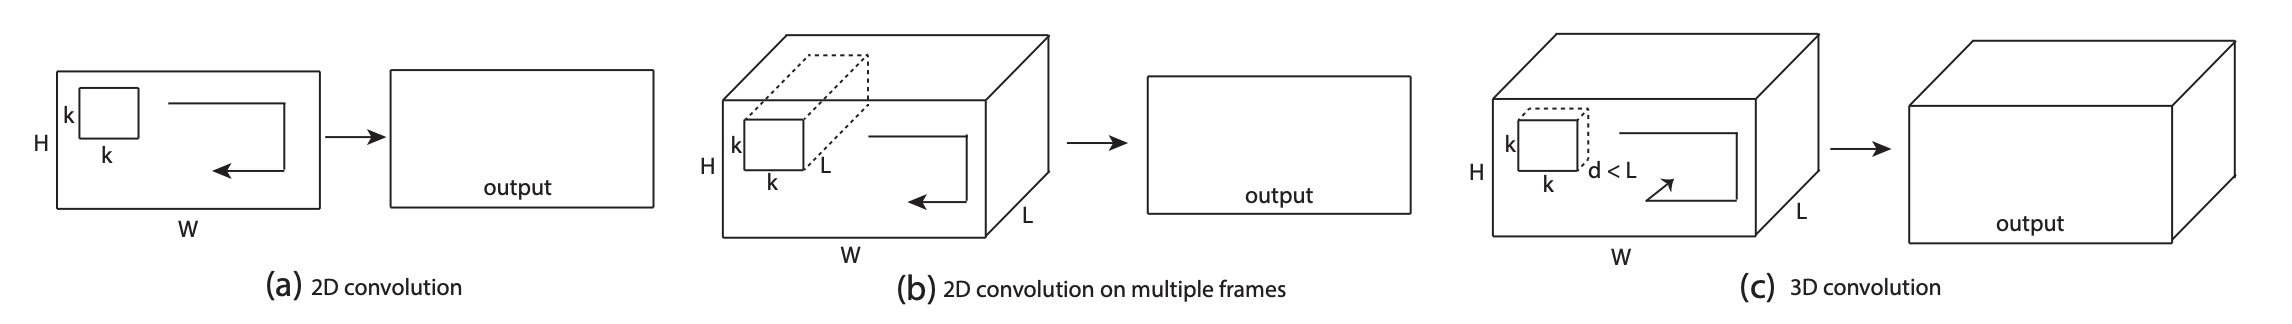
\includegraphics[width=1\textwidth]{images/video_synthesis/conv.png}
    \caption{2D and 3D convolution operations. (a) Applying 2D convolution on image results in an image. (b) Applying 2D convolution on video (multiple frames) also results in an image. (c) Applying 3D convolution on video results in another volume (channel), preserving temporal information. Figure from the 2014 paper \cite{tran2015learning}.}
\end{figure}

A 2014 paper \cite{tran2015learning} by Facebook AI suggested using 3D-ConvNets (3D convolution networks) for video data spatiotemporal feature learning. The dataset that they used are UCF101, Sports-1M, and because Sports-1M has 100x times the amount of video clips compared to UCF101. For each video clip, they extracted five 2-second clips as the train-test split and resized the frames to 128x171, and flipped the frames horizontally with 50\% probability.

Compared to 2D ConvNet, 3D ConvNet has the ability to model temporal information better owing to 3D convolution and 3D pooling operations. The researchers found that 3x3x3 kernel size is the best option for 3D ConvNets. After every 3D convolution layer they apply 3D max-pooling.

\begin{figure}
    \centering
    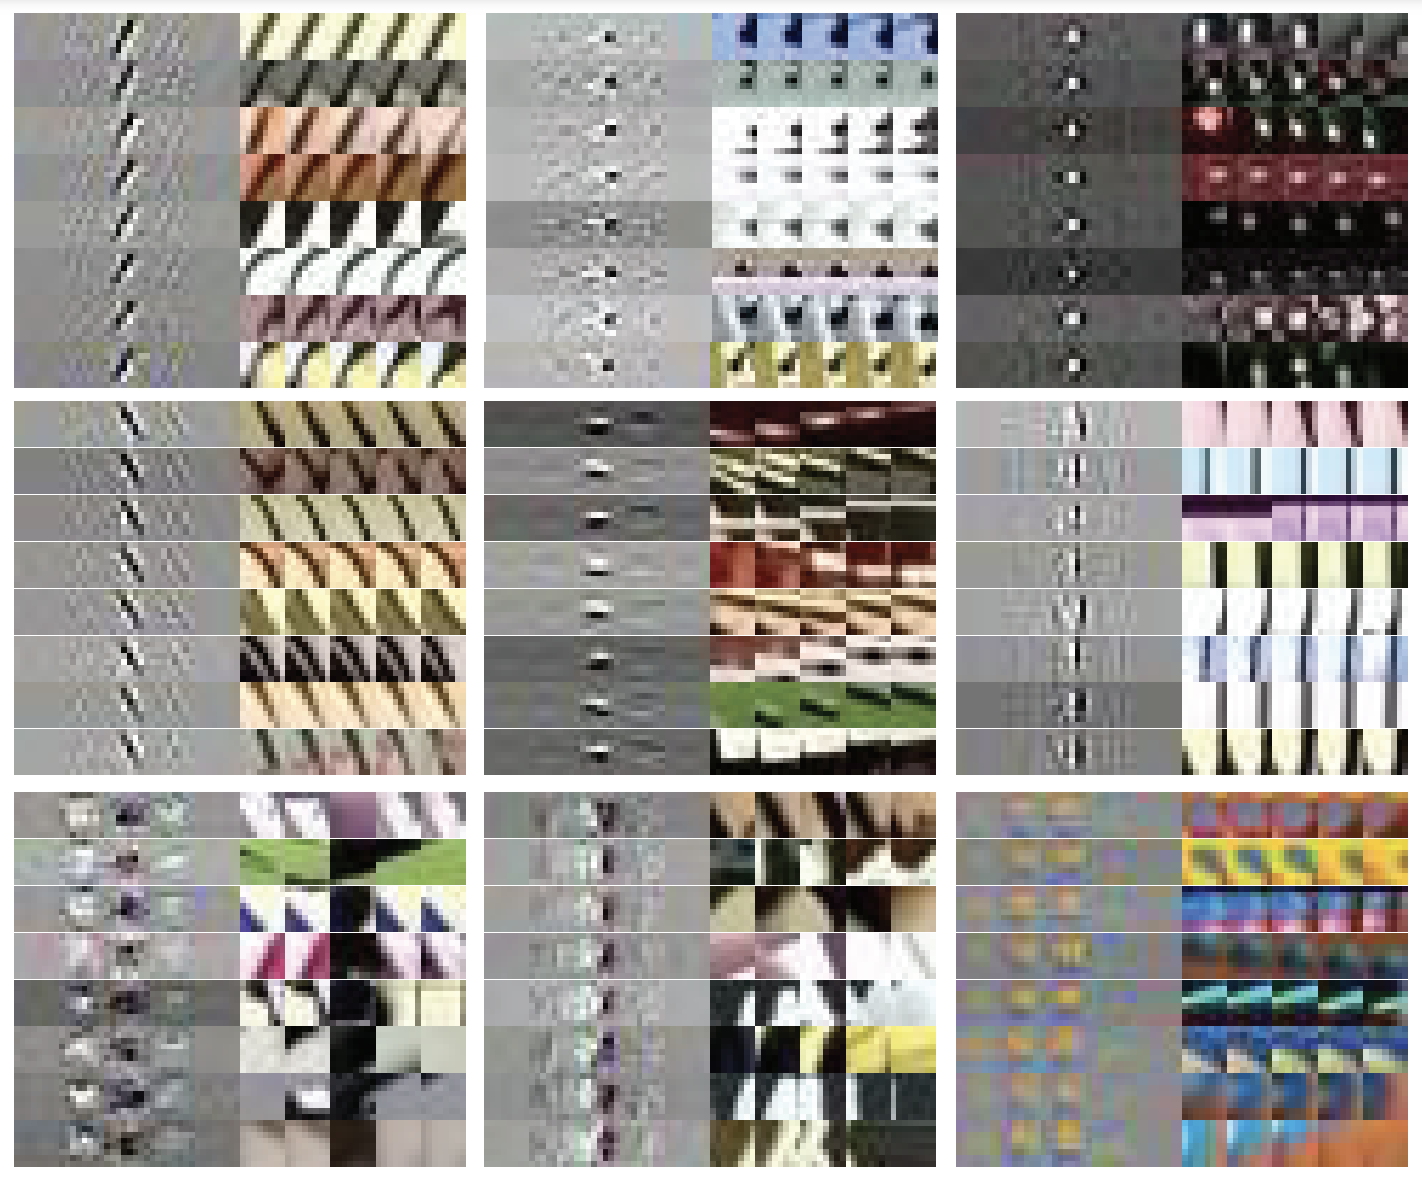
\includegraphics[width=1\textwidth]{images/video_synthesis/c3d_feature_maps.png}
    \caption{Feature maps of the first 3D convolution layer of the C3D model \cite{tran2015learning}. The first two rows of the feature maps shows the detection of moving edges and blobs, while the last row shows edge orientation changes and color changes.}
    \label{fig:c3d_feature_maps}
\end{figure}

Figure \ref{fig:c3d_feature_maps} shows the feature maps of the first 3D convolution layer of the C3D model. The 3D convolution helps to capture motion between frames.

In a 2018 paper \cite{tran2018closer} that reviews spatiotemporal convolution (also by Facebook AI), they observed that 2D CNNs applied on individual frames of video remain solid performers in action recognition (the classification of action [like cooking, running, dancing] in image/video). By using residual connections, and by factorizing the 3D convolutional filters into separate spatial and temporal components results in the creation of a new spatiotemporal convolution block called \texttt{R(2+1)D}. The \texttt{R(2+1)D} block is a 2D residual block followed by a 1D temporal convolution. This separation allows the model to represent more complex non-linear functions, and is more easily optimized.







\subsection{Practices \& techniques in vision domain}

\begin{figure}
    \centering
    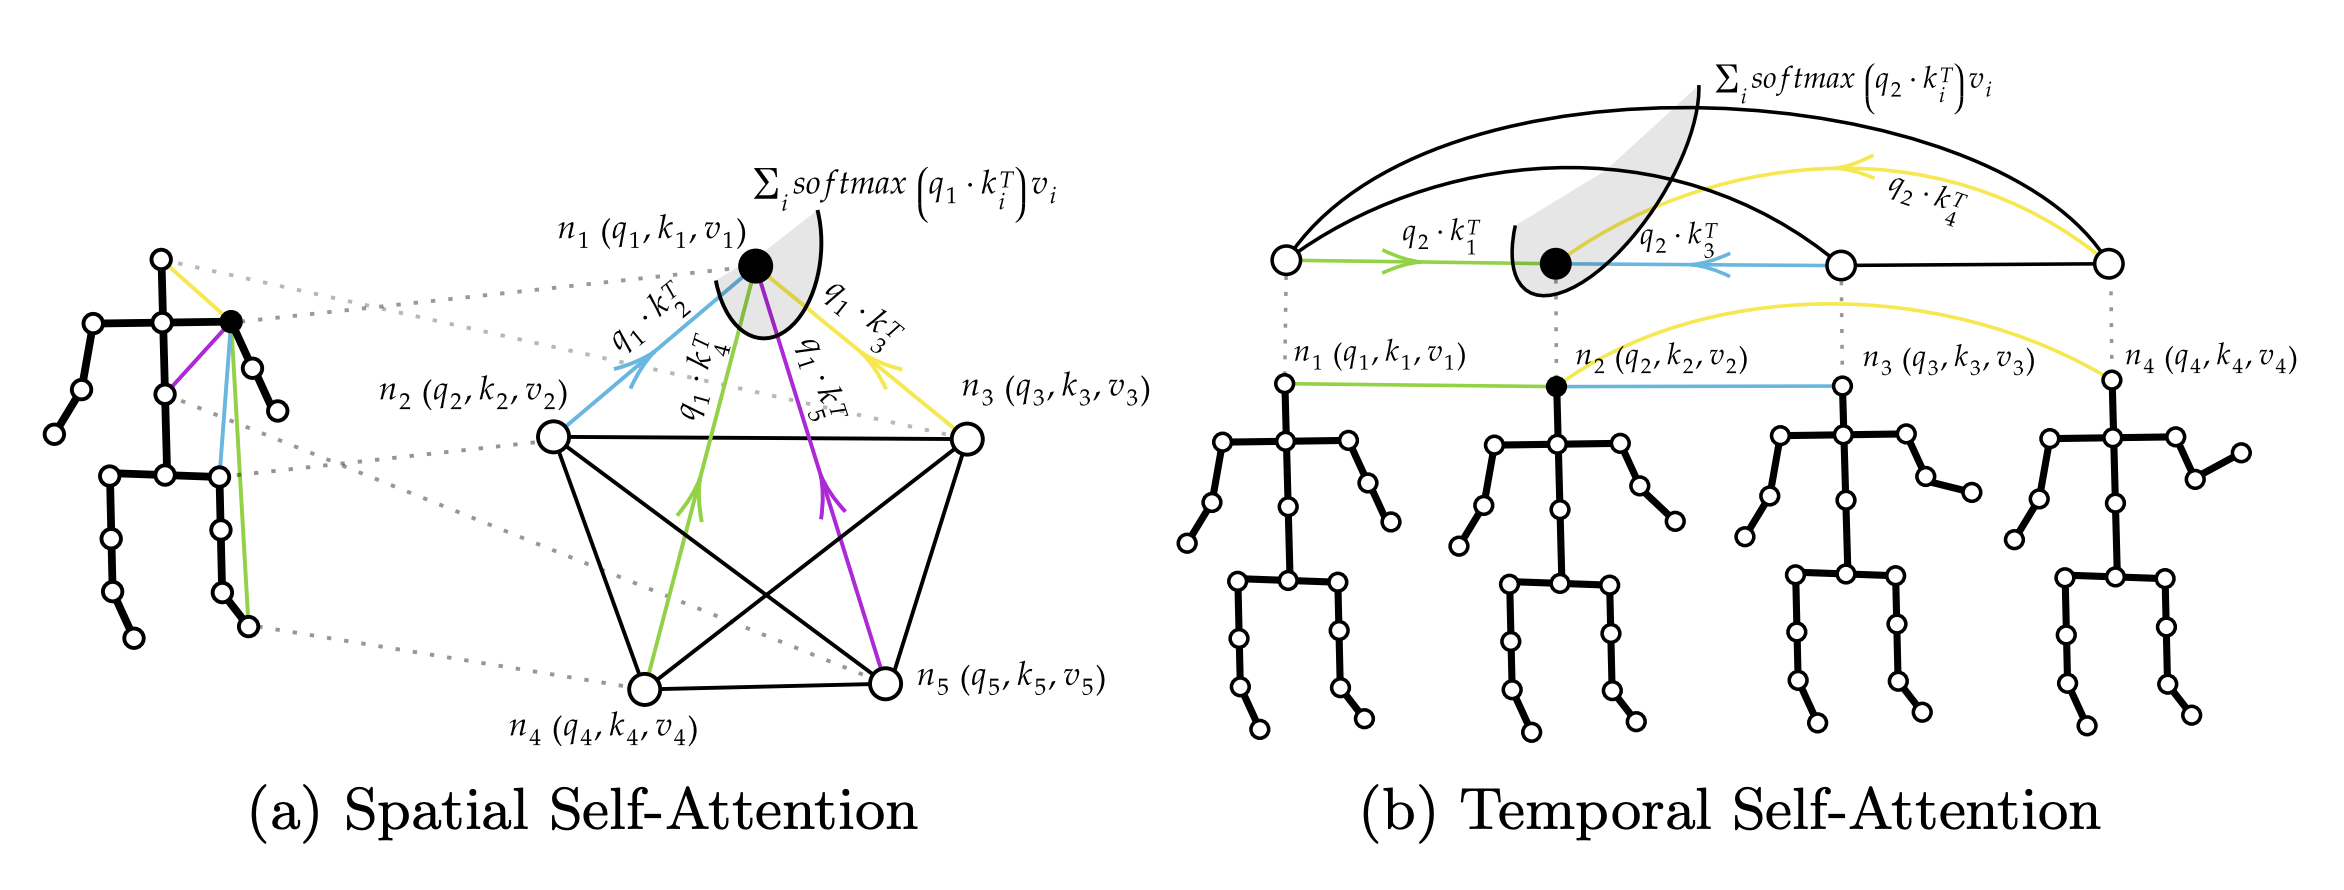
\includegraphics[width=1\textwidth]{images/video_synthesis/spatial_and_temporal_self_attention.png}
    \caption{Spatial and temporal self-attention topology graph illustration \cite{plizzari2021spatial}. The model tries to learn 3D skeleton pose over time. \textit{Left:} full-graph of skeleton joins; spatial self-attention (SSA): the model learns the relations between joints (nodes). \textit{Right:} temporal self-attention (TSA); the dynamics of each joint is studied separately along all the frames, each node is independent and correlations between frames are computed between the same body joints along the temporal dimension.}
    \label{fig:spatial_temporal_self_attention}
\end{figure}

In this section we explore common practices or techniques used in vision domain, that are applied in image synthesis and video synthesis models.

\textbf{Use of transformers for multi-modal outputs:} Transformers have been shown time and time again their capability to scale to very large models. In addition, they excel at sequence-to-sequence tasks, which allows researchers to use them in their vision models and condition on multiple types of data (text, audio, image, layouts, semantic masks, etc). As we advance further into more and more advanced vision models, we see increase in the use of transformers in vision tasks.

\textbf{Patchify:} In Vision Transformer (ViT) \cite{vision_transformer} (appendix \ref{appendix:vision_transformer}) and Diffusion Transformer (DiT) \cite{diffusion_transformer} (appendix \ref{appendix:diffusion_transformer}) both use patch technique to model and represent patches of size $p \times p$ of an image. First the image is divided into patches, then each patch is linearly embedded into a vector, and the position (either absolute, relative or even distance between patches) of the patch is added (element-wise) to the patch embeddings, forming an embedding of patch + position tokens, and then the sequence of tokens is fed into the transformer (in the case of ViT and DiT). 

\textbf{Spatial Self-Attention (SSA):} Self-attention mechanism is often used to capture long-range spatial dependencies in a single frame. Unlike CNNs, which capture only local features, self-attention allows the model to learn the global of an image. Spatial self-attention is used in Vision Transformer (ViT) \cite{vision_transformer} (appendix \ref{appendix:vision_transformer}), for instance.

\textbf{Temporal Self-Attention (TSA):} Self-attention mechanism is also often used to capture temporal dependencies (relationships between frames). For example, it enables the model to understand how each part of the video changes over time, allowing it to learn motion patterns. Video-LDM \cite{video_ldm} (section \ref{sec:videoldm}) for example uses temporal self-attention.

\textbf{Color reduction:} In \cite{imagegpt} they proposed context reduction: first by downsizing the resolution of the training videos to lower resolution, and more importantly, they created their own 9-bit color palette by K-mean clustering (k=512). That means, each pixel is represented by 9 bits, instead of 256x256x256 (which require 8+8+8=24 bits). This color reduction yields a sequence length three times shorter than the standard (R, G, B) palette.

\textbf{Use of compute efficient attention blocks:} Like in the case of Video-GPT they use \textbf{Axial attention} block (appendix \ref{appendix:attention}), which doesn't compute self-attention of the entire image, but only of the rows and columns separately. This reduces the complexity of the attention mechanism.

\textbf{Operating in latent space:} Because video synthesis is compute intensive task, a lot of previous works models operate in latent space, which is compressed lower-dimension space, compared to raw RGB frames. Most of the time, variational autoencoder is used to encode to latent space and the decoder to decode the latent space back to the RGB space.

\textbf{Conditioning mechanisms:} There are three ways to condition an image/video generation model: \textbf{cross-attention} which we saw in stable diffusion, \textbf{adaptive layer normalization} (like in diffusion transformer) and in transformer-based models, the conditional information is added to the \textbf{input sequence tokens} (like in ViT and DiT) to be fed into the transformer decoder.

\textbf{Reusing pre-trained models:} In Video-LDM for instance, they used pre-trained image generator and then converted it to video generator by adding temporal layers. Another example is Imagen where the Google researchers used pre-trained T5-XXL text encoder to encode the text prompts.

\textbf{Inserting temporal layers:} Inserting temporal layers into image synthesis models has been explored by MoCoGAN-HD \cite{mocogan_hd}, StyleVideoGAN \cite{style_video_gan} and Video-LDM \cite{video_ldm} (section \ref{sec:videoldm}). This technique uses pre-trained image generator and then adds temporal layers to the model, which converts the model from image generator to video generator.